%%%%%%%%%%%%%%%%%%%%%%% file template.tex %%%%%%%%%%%%%%%%%%%%%%%%%
%
% This is a general template file for the LaTeX package SVJour3
% for Springer journals.          Springer Heidelberg 2010/09/16
%
% Copy it to a new file with a new name and use it as the basis
% for your article. Delete % signs as needed.
%
% This template includes a few options for different layouts and
% content for various journals. Please consult a previous issue of
% your journal as needed.
%
%%%%%%%%%%%%%%%%%%%%%%%%%%%%%%%%%%%%%%%%%%%%%%%%%%%%%%%%%%%%%%%%%%%
%
% First comes an example EPS file -- just ignore it and
% proceed on the \documentclass line
% your LaTeX will extract the file if required
\begin{filecontents*}{example.eps}
%!PS-Adobe-3.0 EPSF-3.0
%%BoundingBox: 19 19 221 221
%%CreationDate: Mon Sep 29 1997
%%Creator: programmed by hand (JK)
%%EndComments
gsave
newpath
  20 20 moveto
  20 220 lineto
  220 220 lineto
  220 20 lineto
closepath
2 setlinewidth
gsave
  .4 setgray fill
grestore
stroke
grestore
\end{filecontents*}
%
\RequirePackage{fix-cm}
%
%\documentclass{svjour3}                     % onecolumn (standard format)
%\documentclass[smallcondensed]{svjour3}     % onecolumn (ditto)
%\documentclass[smallextended]{svjour3}       % onecolumn (second format)
\documentclass[twocolumn]{svjour3}          % twocolumn
%
\smartqed  % flush right qed marks, e.g. at end of proof
%
\usepackage{graphicx}
\usepackage{color}
\usepackage{amsmath}
\usepackage{amsfonts}
\usepackage{amssymb}
\usepackage{hyperref}
\usepackage{moreverb,url}
\usepackage{xspace}
%\usepackage{algorithmic}
\usepackage{algorithm}
\usepackage[noend]{algpseudocode}
\usepackage{yfonts}

\newcommand\paper{paper\xspace}
\newcommand\partie{section\xspace}
\newcommand\Partie{Section\xspace}
\newcommand\liegroup{\mathcal{L}}
\newcommand\cross[1]{\left[#1\right]_{\times}}
\newcommand\neutral{\mathfrak{n}}
\newcommand\gripper{\mathfrak{g}}
\newcommand\ngrippers{n_{\mathfrak{g}}}
\newcommand\handle{\mathfrak{h}}
\newcommand\nhandles{n_{\mathfrak{h}}}
\newcommand\true{\texttt{true}\xspace}
\newcommand\false{\texttt{false}\xspace}
\newcommand\state{\mathcal{S}}
\newcommand\transition{\mathcal{T}}
\newcommand{\body}{\mathcal{B}}
\newcommand{\CS}{\mathcal{C}}
\newcommand{\conf}{\mathbf{q}}
\newcommand\dconf{\mathbf{\dot{q}}}
\newcommand{\reals}{\mathbb{R}}
\newcommand\entiernaturel{\mathbb{N}}
\newcommand{\fframe}{\mathcal{F}}
\newcommand{\p}{\mathbf{p}}
\newcommand{\x}{\mathbf{x}}
\newcommand{\y}{\mathbf{y}}
\newcommand{\grasps}{\rightarrow}
\newcommand{\isstuckon}{\leftrightarrow}
\newcommand\xx{\mathbf{x}} % \x already defined in the class
\newcommand\nobjects{n_{o}}
\newcommand\object[1]{o_{#1}}
%\newcommand\ngrippers{n_{g}}
%\newcommand\nhandles[1]{n_{h,#1}}
\newcommand\ncontacts[1]{n_{c,#1}}
%\newcommand\gripper[1]{g_{#1}}
%\newcommand\handle[2]{h_{#2,#1}} % handle #1 of object #2
\newcommand\contact[2]{c_{#2,#1}} % contact surface #1 of object #2
\newcommand\grasp[2]{gr(#1,#2)}
\newcommand\placement[1]{pl (#1)}
\newcommand{\roadmap}{\Gamma}
\newcommand\pregrasp{\textit{pregrasp}}
\newcommand\grasplacement{\textit{grasp-placement}}
\newcommand\preplacement{\textit{preplacement}}

\newcommand\trajectory{\Gamma}
\newcommand\task{{T}}
\newcommand\taskSpace{\mathbb{T}}
\newcommand\error{\mathbf{e}}
\newcommand\desired[1]{{#1}^{*}}

\newcommand\ie{\textit{i.e.}}
\newcommand{\manipulationRRT}{\emph{Manipulation RRT}\xspace}
\newcommand{\randomShortcut}{\emph{random shortcut}\xspace}
\newcommand{\trans}{\mathbf{T}}
\newcommand\camera{c}
\newcommand\loc[2]{^{#2}\hat{T}_{#1}}
\newcommand\todo[1]{}

\newcommand\EXTEND{{\scriptsize EXTEND}\xspace}
\newcommand\CONNECT{{\scriptsize CONNECT}\xspace}
\newcommand\TRYCONNECTNEWNODES{{\scriptsize TRY}{\small C}{\scriptsize ONNECT}{\small N}{\scriptsize EW}{\small N}{\scriptsize ODES}\xspace}
\newcommand\TRYCONNECTTOROADMAP{{\scriptsize TRY}{\small C}{\scriptsize ONNECT}{\small T}{\scriptsize O}{\small R}{\scriptsize OADMAP}\xspace}
\newcommand\SETCONSTRAINTS{{\scriptsize SET}{\small C}{\scriptsize ONSTRAINTS}}
\newcommand\ADD{{\scriptsize ADD}}
\newcommand\CREATESTATE{{\scriptsize CREATE}{\small S}{\scriptsize TATE}\xspace}
\newcommand\CREATETRANSITION{{\scriptsize CREATE}{\small T}{\scriptsize RANSITION}\xspace}


%\newtheorem{definition}{Definition}
% Insert the name of "your journal" with
\journalname{Autonomous Robots}
%
\begin{document}

\title{Prehensile Manipulation Planning: Modelling, Algorithms and Implementation}
%\subtitle{Do you have a subtitle?\\ If so, write it here}

%\titlerunning{Algorithmic of manipulation planning}% if too long for running head

\author{Florent Lamiraux         \and
        Joseph Mirabel %etc.
}

%\authorrunning{Short form of author list} % if too long for running head

\institute{F. Lamiraux \at
              LAAS-CNRS \\
              7 avenue du colonel Roche\\
              31077 Toulouse, France\\
              \email{florent.lamiraux@laas.fr}           %  \\
              %             \emph{Present address:} of F. Author  %  if needed
              \and
              J. Mirabel \at
              LAAS-CNRS \\
              7 avenue du colonel Roche\\
              31077 Toulouse, France\\
              \email{joseph.mirabel@laas.fr}           %  \\
}

\date{Received: date / Accepted: date}
% The correct dates will be entered by the editor


\maketitle

\begin{abstract}
\keywords{manipulation planning \and motion planning}
\end{abstract}

\section{Introduction}
This \paper describes a software platform taylored for manipulation planning.
The main contributions are:
\begin{itemize}
\item an original and general implementation of prehensile manipulation based on
  non-linear constraints,
\item an original solver for non-linear constraints that is able to handle implicit and explicit constraints,
\item a manipulation planning algorithm that is able to tackle a great variety of manipulation planning problems,
\item an open-source software suite that implements all the above following state of the art development tools and methods.
\end{itemize}

The \paper is organized as follows.
\partie~\ref{partie:preliminary} introduces some preliminary notions like kinematic chains and Lie groups that are used to model the configuration space of each joint.

Each \partie is implemented by one or several software packages. Instead of providing formulas for some values need to be computed, we provide a link to the C++ implementation.

\section{Preliminaries}\label{partie:preliminary}
\subsection{Kinematic chains and Lie groups}

A kinematic chain is commonly understood as a set of rigid-body links connected
to each other by joints. Each joint has one degree of freedom either in
rotation or in translation. A configuration of the kinematic chain is represented by a vector. Each component of the vector represents the angular or linear value of the correspondig joint.

This representation although well suited for fixed base manipulator
arms is not well adapted for robots with a mobile base like wheeled
mobile robots, aerial robots or legged robots, since the mobility of the base
cannot be correctly represented by translation or rotation joints.
Representing a freeflying object by three virtual translations followed by
three virtual rotations called roll, pitch and yaw is indeed a poor workaround.

\subsubsection{Kinematic chain}

A \textit{kinematic chain} is a tree of \textit{joints} where each
joint represents a mobility of a rigid-body link with respect to
another link or with respect to the world reference frame. To each joint is
associated a configuration space called the \textit{joint configuration space}.
The most common joints with their respective configuration spaces are
\begin{itemize}
\item linear \textit{translation} with configuration space $\reals$,
\item bounded \textit{rotation} with configuration space  $\reals$,
\item unbounded \textit{rotation} with configuration space  $SO(2)$,
\item \textit{planar} with configuration space $SE(2)$,
\item \textit{freeflyer} with configuration space $SE(3)$.
\end{itemize}
$SO(n)$ and $SE(n)$ respectively stand for \textit{special orthogonal group} and \textit{special Euclidean group}. They represents the group of rigid-body transformations and the group of rotations in $\reals^n$.

\subsubsection{Lie groups}

The joint configuration spaces enumerated in the previous paragraph: $\mathbb{R}^n$, $SE(n)$ are all Lie groups. The group operation is $+$ for $\mathbb{R}^n$, and composition denoted as $"."$ for $SE(n)$. We refer to~\cite{LMS94} -- Appendix A for a thorough definition of Lie groups. We expose here only properties that are useful for the sequel of the \paper.

For any Lie group $\liegroup$ with neutral element $\neutral$, the tangent space at the neutral element $T_{\neutral}\liegroup$ of the group naturally maps to the tangent space at any point of the group. This means that any \textit{velocity} $\mathbf{v}\in T_{\neutral}\liegroup$ uniquely defines
\begin{enumerate}
\item a velocity $\mathbf{w}\in T_{g}\liegroup$ at any point $g$ of the group, and thus,
\item a vector field on the tangent space $T\liegroup$, and
\item by integration during unit time of the latter vector field, starting from the origin, a new point $g_{1}\in\liegroup$.
\end{enumerate}
Item 1 above is called the \textit{transport} of velocity $\mathbf{v}$ to $g$.
Item 3 above is called the exponential map of $\liegroup$ and is denoted by $\exp$.

\paragraph{Geometric interpretations}
\begin{itemize}
\item $\reals$ (and by trivial generalization $\reals^n$): the neutral element is $0$. The tangent space at 0 is isomorphic to $\reals$ and
  $$
  \forall \theta\in\reals,\  \exp(\theta) = \theta.
  $$
\item $SE(3)$: an element $g$ of $SE(3)$ can be seen as the position of a moving frame in a fixed reference frame. A point $\mathbf{x}\in\reals^3$ is mapped to $g(\mathbf{x})$. Note that $\mathbf{x}$ is also the coordinate vector of $g(\mathbf{x})$ in the moving frame $g$. If $\mathbf{v}$, $\omega$ are a linear and an angular velocities at the origin, $(\mathbf{v},\omega)$ is transported to $g$
  as the same linear and angular velocities expressed in the moving frame. In other words, if
  \begin{equation}\label{eq:homogeneous matrix}
  M=\left(\begin{array}{ll} R & \mathbf{t}\\ 0 & 1\end{array}\right)
    \end{equation}
  with $R\in SO(3)$ and $\mathbf{t}\in\reals^3$  is the homogeneous matrix
  representing $g$, and $(\mathbf{v},\mathbf{\omega})$ is a velocity in $T_{I_3}SE(3)$, the velocity transported to $g$ corresponds to the linear velocity $R\mathbf{v}$ and $R\omega$ of the moving frame.
  Integral curves of the vector field mentioned in item 2 above correspond to helicoidal motions of constant velocity expressed in the moving frame.
\end{itemize}
$SE(2)$, $SO(3)$, and $SO(2)$ are (or are isomorphic to) subgroups of $SE(3)$ and follow the same geometrical interpretation.

\paragraph{Vector representations}
Each Liegroup element is represented by a vector. Rotations are represented by
unit quaternions.

Therefore elements of $SE(3)$ are represented by a vector in $\reals^7$ where the 3 first components represent the image of the origin (vector $\mathbf{t}$ in Equation~\ref{eq:homogeneous matrix}), the 4 last components represent a unit quaternion.

Elements of $SO(3)$ are represented by a unit vector of dimension 4.

Elements of $SE(2)$ are represented by a vector of dimension 4. The 2 first components represent the image of the origin. The 2 last components represent the cosine and sine of the rotation angle. Therefore the homogeneous matrix associated to $\conf=(q_1,q_2,q_3,q_4)$ is
$$
M = \left(\begin{array}{lll}
  q_3 & -q_4 & q_1 \\
  q_4 &  q_3 & q_2 \\
  0   &  0  & 1
\end{array}\right).
$$
Table~\ref{tab:vector representation} compiles this information.
\begin{table}
  \begin{tabular}{|l|c|c|}
    \hline
    Lie group type & configuration & velocity\\
    \hline
    $SE(3)$ & $(x_1,x_2,x_3,p_1,\cdots,p_4)$ & $\dconf=(\mathbf{v},\omega)$ \\
            & $\in\reals^7$                 & $\in\reals^6$ \\
    $SE(2)$ & $(x_1,x_2,\cos\theta,\sin\theta)$ & $\dconf=(\mathbf{v},\dot{\theta})$\\
            & $\in\reals^4$                 & $\in\reals^3$ \\
    $SO(3)$ & $(p_1,p_2,p_3,p_4)\in\reals^4$ & $\dconf=\omega\in\reals^3$\\
    $SO(2)$ & $(\cos\theta,\sin\theta)\in\reals^2$ & $\dconf=\dot{\theta}\in\reals$\\
    \hline
  \end{tabular}
  \caption{Main Lie group types and their vector representations. Notice that the dimensions of the configuration representation and of the velocity representation may differ.}
  \label{tab:vector representation}
\end{table}

\paragraph{Exponential map}

As expressed earlier, following a constant velocity $\dot{\conf}$ from the neutral element of a joint configuration space leads to another configuration denoted as
$$
\conf = \exp(\dconf).
$$
In some cases, we may specify in subscript the Lie group that is used: \href{https://github.com/stack-of-tasks/pinocchio/blob/f8f3b9a24eab527df79650e3dc73410f9a46a2b2/src/spatial/explog.hpp#L34}{$\exp_{SO(3)}$}, \href{https://github.com/stack-of-tasks/pinocchio/blob/f8f3b9a24eab527df79650e3dc73410f9a46a2b2/src/spatial/explog.hpp#L236}{$\exp_{SE(3)}$}.

For all Lie groups $\reals$, $SO(n)$, $SE(n)$, the exponential map is surjective. This means that for any $\conf\in\liegroup$, there exists $\mathbf{v}\in T_{\neutral}\liegroup$, such that $\conf = \exp(\mathbf{v})$.
Although $\exp$ is not injective, choosing the smallest norm $\mathbf{v}$ uniquely defines function $\log$ from $\liegroup$ to $T_{\neutral}\liegroup$, up to some singularities where several candidates $\mathbf{v}$ are of equal norms.
Again, we may specify the Lie group that is used: \href{https://github.com/stack-of-tasks/pinocchio/blob/f8f3b9a24eab527df79650e3dc73410f9a46a2b2/src/spatial/log.hxx#L112}{$\log_{SE(3)}$}, \href{https://github.com/stack-of-tasks/pinocchio/blob/f8f3b9a24eab527df79650e3dc73410f9a46a2b2/src/spatial/log.hxx#L15}{$\log_{SO(3)}$}

\paragraph{Sum and difference notations}

Following a constant velocity $\dconf\in T_{\neutral}\liegroup$ starting from $\conf_0\in\liegroup$, leads to
$$
\conf_1 = q_0.\exp(\dconf).
$$
Note that if $\liegroup=\reals$, we write
$$
\conf_1 = \conf_0 + \dconf,
$$
since the Lie group operator of $\reals$ is $+$ and $\exp_{\reals}$ is the identity.
In order to homogeneize notation, we define the following operators:
\begin{eqnarray}\label{eq:plus}
  \conf_0 \oplus \dconf &\triangleq& \conf_0.\exp(\dconf),\\
  \label{eq:minus}
  \conf_1 \ominus \conf_0 &\triangleq& \log(\conf_0^{-1}.\conf_1).
\end{eqnarray}

\subsubsection{Robot configuration space}

Given a kinematic chain with joints $(J_1, \cdots, J_{njoints})$, ordered in such
a way that each joint has an index bigger than its parent in the tree, the configuration space of the robot is the cartesian product of the joint configuration spaces.
$$
\CS \triangleq \CS_{J_1}\times \cdots \times \CS_{J_{njoints}}.
$$
$\CS$ naturally inherits the Lie group structure of the joint configuration spaces through the Cartesian product.
We denote by $nq_i$, $nv_i$ the sizes of the configuration and velocity vector representations of joint $J_i$, as defined in Table~\ref{tab:vector representation}.
The configuration and velocity of the robot can thus be represented by vectors of size $nq$ and $nv$ such that
$$
nq = \sum_{i=1}^{njoints} nq_i, \ \ \ nv = \sum_{i=1}^{njoints} nv_i
$$
We denote by $iq_i$, and $iv_i$ the indices of joint $i$ in the robot configuration and velocity vectors.
$$
iq_i = \sum_{j=1}^{i-1} nq_j\ \ \ \ iv_i = \sum_{j=1}^{i-1} nv_j
$$
With these definitions and notation, the linear interpolation between two robot
configurations $\conf_0$ and $\conf_1$ is naturally written:
$$
\conf(t) = \conf_0 \oplus t (\conf_1 - \conf_0)
$$
This formula generalizes the linear interpolation to robots with freeflying bases, getting rid of singularities of roll -- pitch -- yaw parameterization.
%% begin impl
Cartesian products of Lie groups are represented by class \href{https://gepettoweb.laas.fr/hpp/hpp-pinocchio/doxygen-html/classhpp_1_1pinocchio_1_1LiegroupSpace.html}{\texttt{LiegroupSpace}}. Elements of these spaces are represented by classes
\begin{itemize}
\item \href{https://gepettoweb.laas.fr/hpp/hpp-pinocchio/doxygen-html/classhpp_1_1pinocchio_1_1LiegroupElementBase.html}{\texttt{LiegroupElement}}
\item \href{https://gepettoweb.laas.fr/hpp/hpp-pinocchio/doxygen-html/classhpp_1_1pinocchio_1_1LiegroupElementBase.html}{\texttt{LiegroupElementRef}}, and
\item \href{https://gepettoweb.laas.fr/hpp/hpp-pinocchio/doxygen-html/classhpp_1_1pinocchio_1_1LiegroupElementBase.html}{\texttt{LiegroupElementConstRef}}.
  \end{itemize}
%% end impl

\section{Non-linear constraints and solvers}

Some tasks require the robot to enforce some non-linear constraints. Foot contact on the ground for a humanoid robot, center of mass projection on a horizontal plane, gaze constraint are a few examples.

\subsection{Non-linear constraints}

\begin{definition}\textbf{Non-linear constraint.} A non linear constraint is defined by a differentiable mapping $h$ from $\CS$ to a vector space $\reals^m$ and is written
\begin{equation}\label{eq:constraint}
h(\conf) = 0.
\end{equation}
\end{definition}
If the robot is subject to several numerical constraints, $h_1,\cdots,h_k$ with values in $\reals^{m_1}\cdots\reals^{m_k}$, these constraints are equivalent to a single constraint $h$ with values in $\reals^{m}$, where $m=\sum_{i=1}^k m_i$, such that
$$
h(\conf) \triangleq \left(\begin{array}{c} h_1(\conf) \\ \vdots \\ h_k(\conf)
\end{array}\right).
$$
It may be useful to use a non zero right hand side for the same function $h$. We define for that parameterized non-linear constraints.
\begin{definition}\textbf{Parameterized non-linear constraints.}
  A parameterized non-linear constraint is defined by a differentiable mapping $h$ from $\CS$ to a vector space $\reals^m$ and by a vector $\mathbf{h}_0$ of $\reals^m$ and is written
  $$
  h(\conf) = \mathbf{h}_0.
  $$
\end{definition}
%% begin impl
Differentiable functions are represented by class\\ \href{https://gepettoweb.laas.fr/hpp/hpp-constraints/doxygen-html/classhpp_1_1constraints_1_1DifferentiableFunction.html}{\texttt{DifferentiableFunction}}.
%% end impl

\paragraph{Jacobian}

In this \paper, we will make use of the term Jacobian in a generalized way.
If $h$ is a differentiable function from a Lie group $\liegroup_1$ to a Lie group $\liegroup_2$, and $\conf_1$ an element of $\liegroup_1$, we will denote by $\frac{\partial h}{\partial\conf}(\conf_1)$ the operator that maps velocities in $T_{\conf_1}\liegroup_1$ to the corresponding velocity of the image by $h$ in $T_{h(\conf_1)}\liegroup_2$.

This operator is represented by a matrix with $nv_2$ lines and $nv_1$ columns, where $nv_1$ and $nv_2$ are the dimensions of the tangent spaces of respectively $\liegroup_1$ and $\liegroup_2$.

\subsection{Newton based solver}

It is sometimes useful to produce a configuration $\conf$ that satisfies a constraint (or a set of constraints) of type~(\ref{eq:constraint}) from a configuration $\conf_0$ that does not. This action is called the \textit{projection of $\conf_0$ onto the submanifold defined by the constraint} and is performed by a numerical solver that iteratively linearizes the constraint as follows:
$$
h(\conf_{i+1}) \approx h(\conf_i) + \frac{\partial h}{\partial \conf}(\conf_{i})(\conf_{i+1}-\conf_i) = 0
$$
Iterate $\conf_{i+1}$ is computed as follows:
\begin{equation}\label{eq:HierarchicalIterative}
\conf_{i+1} = \conf_i-\alpha_i\frac{\partial h}{\partial \conf}^{+}(\conf_{i}) h(\conf_i)
\end{equation}
where $.^{+}$ denotes the Moore Penrose pseudo inverse, and $\alpha_i$ is a positive real number called the step size. Taking $\alpha_i=1$ exactly solves the linear approximation, but it may not be the best choice in general.

The computation of $\alpha_i$ is performed by a line search algorithm.
The algorithm stops when the norm of each $h_i(\conf_{i+1})$ is below a given error threshold.
%% begin impl
Class\\ \href{https://gepettoweb.laas.fr/hpp/hpp-constraints/doxygen-html/classhpp_1_1constraints_1_1solver_1_1HierarchicalIterative.html}{\texttt{HierarchicalIterative}} implements the above Newton method. Several linesearch methods are implemented: \href{https://gepettoweb.laas.fr/hpp/hpp-constraints/doxygen-html/structhpp_1_1constraints_1_1solver_1_1lineSearch_1_1Backtracking.html}{\texttt{Backtracking}}, \href{https://gepettoweb.laas.fr/hpp/hpp-constraints/doxygen-html/structhpp_1_1constraints_1_1solver_1_1lineSearch_1_1ErrorNormBased.html}{\texttt{ErrorNormBased}}, \href{https://gepettoweb.laas.fr/hpp/hpp-constraints/doxygen-html/structhpp_1_1constraints_1_1solver_1_1lineSearch_1_1FixedSequence.html}{\texttt{FixedSequence}}, and \href{https://gepettoweb.laas.fr/hpp/hpp-constraints/doxygen-html/structhpp_1_1constraints_1_1solver_1_1lineSearch_1_1Constant.html}{\texttt{Constant}}.
Note that to define a new constraint, the user needs to derive class \href{https://gepettoweb.laas.fr/hpp/hpp-constraints/doxygen-html/classhpp_1_1constraints_1_1DifferentiableFunction.html}{\texttt{DifferentiableFunction}} and to implement methods \texttt{impl\_compute} and \texttt{impl\_jacobian}.
%% end impl

\subsection{Explicit constraints}

In manipulation planning applications, where robots manipulate objects, once an object is grasped, the position of the object can be computed explicitely from the configuration of the robot. In this case, some configuration variables of the system depends on other:
$$
\conf=(\conf_{rob},\conf_{obj})\in\CS,\ \ \ \ \conf_{obj} = g_{grasp}(\conf{rob}).
$$
Although this constraint may fit definition~(\ref{eq:constraint}) by defining
\begin{equation}\label{eq:explicit-grasp}
h(\conf) \triangleq \conf_{obj} \ominus g_{grasp}(\conf_{rob}),
\end{equation}
solving this constraint possibly with other constraints using an iterative scheme~(\ref{eq:HierarchicalIterative}) is obviously sub-optimal.
Notice that the right hand side of~(\ref{eq:explicit-grasp}) is the $\log$ of the pose of the object when grasped, with respect to the actual pose of the object.

More generally, let us denote by
\begin {itemize}
\item $I_{nq}$ the set of positive integers not greater than $nq=\dim\CS$,
\item $I$ a subset of $I_{nq}$,
\item $\bar{I}$ the complement in $I_{nq}$ of $I$,
\item $|I|$ the cardinal of $I$.
\end {itemize}
If $\conf\in\CS$ is a configuration, we denote by $\conf_{I}\in\reals^{|I|}$ the vector composed of the components of $\conf$ of increasing indices in $I$.
\paragraph {Example} if $\conf = (q_1,q_2,q_3,q_4,q_5,q_6,q_7)$ and $I=\{1,2,6\}$, then $\conf_I=(q_1,q_2,q_6)$, $\conf_{\bar{I}}=(q_3,q_4,q_5,q_7)$.

Similarly, if
\begin{itemize}
\item $m$ and $n$ are two integers,
\item $M$ and $N$ are two subsets of respectively $I_{m}$ and $I_{n}$,
\item $J$ is a matrix with $m$ rows and $n$ columns,
\end{itemize}
we denote by
\begin{equation}\label{eq:sub-matrix}
  J_{M,N}
\end{equation}
the matrix of size $|M| \times |N|$ obtained by extracting the rows of $J$ of indices in $M$ and the columns of $J$ with indices in $N$.

\paragraph{Example}
If $m=3$, $n=4$, $M=\{2,3\}$ and $N=\{1,2,4\}$,
$$
J = \left(\begin{array}{cccc}
  J_{1,1} &   J_{1,2} &   J_{1,3} &   J_{1,4}\\
  J_{2,1} &   J_{2,2} &   J_{2,3} &   J_{2,4}\\
  J_{3,1} &   J_{3,2} &   J_{3,3} &   J_{3,4}\\
  J_{4,1} &   J_{4,2} &   J_{4,3} &   J_{4,4}
\end{array}\right)
$$
then
$$
J_{M\times N} = \left(\begin{array}{ccc}
  J_{2,1} &   J_{2,2} &   J_{2,4}\\
  J_{3,1} &   J_{3,2} &   J_{3,4}
\end{array}\right)
$$
  
\begin{definition}\label{def:Explicit}
An explicit constraint $E=(in, out, f)$ is a mapping from $\CS$ to $\CS$, defined by the following elements:
\begin{itemize}
\item a subset of input indices $in\subset\{1,\cdots, nq\}$,
\item a subset of output indices $out\subset\{1,\cdots, nq\}$,
\item a smooth mapping $f$ from $\reals^{|in|}$ to $\reals^{|out|}$,
\end{itemize}
satisfying the following properties:
\begin{itemize}
\item $in\cap out = \emptyset$,
\item for any $\p\in\CS$, $\conf = E(\p)$ is defined by
  \begin{align*}
    &\conf_{\bar{out}} = \p_{\bar{out}}\\
    &\conf_{out} = f (\p_{in}).
  \end{align*}
\end{itemize}
\end{definition}

\subsection{Solver by substitution}

To optimize constraint resolution, we perform variable substitution when possible in order to reduce both the number of variables and the dimension of the resulting implicit constraint. We describe here the method that has been first published in~\cite{mirabel:hal-01804774}. Unlike in the former paper, the description we give in Algorithm~\ref{alg:ExplicitConstraintSet} is closer to the real implementation. Some links to the source code are indeed provided in the algorithm description.
\begin{algorithm}
  \begin{algorithmic}[1]
    \Procedure{initializeSolver}{}
    \State{$explicit$} $\gets$ empty vector of explicit constraints
    \State{$nc \gets 0$}
    \State{$args \gets$ array of size $nq$ filled with -1}
    \EndProcedure
    \Function{add}{$E=(in, out, f)$}
    \If{$args_{out}$ contains an element $\geq 0$}
    \State{return failure}
    \EndIf
    \State{queue $idxArg \gets$ elements of $in$}
    \While{$idxArg$ \textbf{not} empty}
    \State{$iArg \gets idxArg$ first element}
    \State{remove $idxArgs$ first element}
    \If{$iArg\in out$}
    \State{return failure}
    \EndIf
    \If{$args[iArg] == -1$}
    \State{continue}
    \Else
    \State{push $explicit[args[iArg]].in$ elements into $idxArg$}
    \EndIf
    \EndWhile
    \State{fill $args_{out}$ with $nc$}
    \State{explicit.add($E$); $nc\gets nc+1$}
    \State{computeOrder()}
    \State{\Return{success}}
    \EndFunction
  \end{algorithmic}
  \caption{Insertion of an explicit constraint in the solver. Line 1 is called once at initialization of the solver. $explicit$ is a vector that stores the constraints that are successfully added to the solver. $nc$ is the size of the latter. $args$ is an array that stores for each configuration variable, the index in $explicit$ of the constraint that computes this configuration variable, -1 if no constraints computes the index. Procedure \href{https://github.com/humanoid-path-planner/hpp-constraints/blob/2555dfec945575f824bd973c30c5c13ec3b67645/src/explicit-constraint-set.cc\#L144}{ADD} tests whether explicit constraint $E$ is compatible with the previously inserted constraints. Line 6 checks whether any output variable of $E$ is already computed by a previous explicit constraint. If so the procedure returns failure and the $E$ is not inserted. The Loop at line 9 recursively checks that any element of $out$ is not an input variable of a previously inserted constraint. If the loop ends without returning failure,  line 18 stores that elements of $out$ are computed by $E$ and $E$ is inserted in vector of constraints. Function \href{https://github.com/humanoid-path-planner/hpp-constraints/blob/2555dfec945575f824bd973c30c5c13ec3b67645/src/explicit-constraint-set.cc\#L301}{computeOrder} at line 20 recursively computes the order in which the explicit constraints are evaluated, following the rule that the input of a constraint should be evaluated before the output.}
  \label{alg:ExplicitConstraintSet}
\end{algorithm}
Once several compatible explicit constraints have been inserted in the solver,
they behave as a single one. For instance, if $\conf=(\conf_1,\conf_2,\conf_3)$,
$$
  \left\{\begin{array}{lcl}\conf_1 &=& f_1(\conf_2)\\
  \conf_2 &=& f_2(\conf_3)\end{array}\right. \mbox{ becomes }
  \left[\begin{array}{cc}\conf_1\\ \conf_2\end{array}\right] =
    \left[\begin{array}{cc}f_1(f_2(\conf_3))\\ f_2(\conf_3)\end{array}\right],
$$
and $f_2$ should be evaluated before $f_1$.

\paragraph{Substitution} When an explicit constraint is not successfully added following Algorithm~\ref{alg:ExplicitConstraintSet}, it is handled as an implicit constraint. Therefore, after inserting implicit and explicit constraints, the solver stores a system of equations equivalent to one explicit and one implicit constraints that we denote by:
\begin{eqnarray}\label{eq:substitution-1}
  h(\conf_{in},\conf_{out}) &=& 0, \\
  \label{eq:substitution-2}
  \conf_{out} &=& f(\conf_{in}), \mbox{ where }\\
  \label{eq:substitution-3}
  \conf &=& (\conf_{in},\conf_{out}).
\end{eqnarray}
Substituting~(\ref{eq:substitution-2}) into~(\ref{eq:substitution-1}), we define an implicit constraint on $\conf_{in}$ only:
$$
\tilde{h}(\conf_{in}) \triangleq h(\conf_{in}, f(\conf_{in})) = 0
$$
The \textit{solver by substitution} applies iteration~(\ref{eq:HierarchicalIterative}) to $\tilde{h}$, instead of $h$. We need therefore to compute the Jacobian of  $\tilde{h}$:
$$
\frac{\partial \tilde{h}}{\partial \conf_{in}}  =
\frac{\partial h}{\partial \conf_{in}} + \frac{\partial h}{\partial \conf_{out}}.
\frac{\partial f}{\partial \conf_{in}}.
$$
As the Jacobian of $h$ is provided with the implicit constraint, we need to compute $\frac{\partial f}{\partial \conf_{in}}$. Let us recall that $f$ may be the combination of several compatible explicit constraints. Let us denote by $E$ the mapping from $\CS$ to $\CS$ associated to $f$ by Definition~\ref{def:Explicit}.
Let $J$ denote the $nv\times nv$ Jacobian matrix of $E$. Then $J$ is defined by blocks as follows:
\begin{equation}\label{eq:jacobian-explicit}
\begin{array}{cc}
  J_{{in}\times{in}} = I_{|{in}|} & J_{{in}\times{out}} = 0 \\
  J_{{out}\times{in}} = \frac{\partial f}{\partial \conf_{in}} & J_{{out}\times{out}} = 0
\end{array}
\end{equation}
If $E$ is the composition of several explicit constraints $E_i=(in_i,out_i,f_i)$ of Jacobian $J_i$, $i\in I_{nc}$, for an integer $nc$, then
\begin{equation}\label{eq:jacobian-product}
J = \prod_{i=nc}^{1} J_{i},
\end{equation}
with $J_i$ obtained by expression~(\ref{eq:jacobian-explicit}) after replacing $in$, $out$, and $f$ by $in_i$, $out_i$, and $f_i$.

$\frac{\partial f}{\partial\conf_{in}}$ is then obtained by extracting from $J$ block $out\times in$.

Let us now detail the iterative computation of~(\ref{eq:jacobian-product}). Let $J$ be the product of of $J_j$ for $j$ from $nc$ to $i+1$.
Note that if $J_i$ and $J$ are square matrices of size $nv$, of the form~(\ref{eq:jacobian-explicit}), $J_i.J$ can be computed by block as follows:
\begin{eqnarray*}
  (J_{i}.J)_{in_{i}\times I_{nv}} &=& J_{in_{i}\times I_{nv}}\\
  (J_{i}.J)_{out_{i}\times I_{nv}} &=& \frac{\partial f_i}{\partial\conf_{in_{i}}}.J_{in_{i}\times I_{nv}}\\
\end{eqnarray*}
and as columns $out$ of $J$ are equal to $0$, left multiplying $J$ by $J_i$ consists in modifying only the following block of $J$:
$$
  (J_{i}.J)_{out_{i}\times in} = \frac{\partial f_i}{\partial\conf_{in_{i}}}.J_{in_{i}\times {in}}\\
$$
Other coefficients of $J_{i}J$ are equal to the corresponding coefficients of $J$.
An implementation of the above Jacobian product can be found \href{https://github.com/humanoid-path-planner/hpp-constraints/blob/e21490c8c713949bd3038dccb6fe02cf254a615f/src/explicit-constraint-set.cc#L267}{here}.

% begin impl
The solver by substitution described in this section is implemented by class \href{https://gepettoweb.laas.fr/hpp/hpp-constraints/doxygen-html/classhpp_1_1constraints_1_1solver_1_1BySubstitution.html}{\texttt{SolverBySubstitution}}, that store an instance of \href{https://gepettoweb.laas.fr/hpp/hpp-constraints/doxygen-html/classhpp_1_1constraints_1_1ExplicitConstraintSet.html}{\texttt{ExplicitConstraintSet}}.

\paragraph{Important remark} As mentioned in Table~\ref{tab:vector representation}, the configuration and velocity vectors may have different sizes. As a consequence, index sets $in$ and $out$ in Definition~\ref{def:Explicit} correspond to configuration vector indices, while in Expression~(\ref{eq:jacobian-explicit}) they correspond to velocity vector indices. To keep notation simple, we use the same notation for different sets.

\subsection{Constrained path}

Now that we are able to project configurations onto submanifolds defined by numerical constraints -- up to some numerical threshold, we need now to define paths on such submanifolds. The usual way of doing so is to discretize the path and to project each sample configuration. The shortcoming of this method is that is requires to choose a discretization step at path construction and to lose the continuous information of the path.

Instead, we propose an alternative architecture where paths store the constraints they are subject to and apply the constraints at path evaluation. Let $P\in C^1([0,T],\CS)$ be a path without constraint defined on an interval $[0,T]$, and $\mathbf{proj}$ a projector onto a submanifold defined by numerical constraints (\textit{i.e.} an instance of\\ \href{https://gepettoweb.laas.fr/hpp/hpp-constraints/doxygen-html/classhpp_1_1constraints_1_1solver_1_1BySubstitution.html}{\texttt{SolverBySubstitution}}).

Then the corresponding constrained path $\tilde{P}$ is defined on the same interval by
$$
\forall t\in[0,T],\ \ \ \tilde{P}(t) = \mathbf{proj}(P(t))
$$
Paths are implemented by class \href{https://gepettoweb.laas.fr/hpp/hpp-core/doxygen-html/classhpp_1_1core_1_1Path.html}{\texttt{Path}}. Several implementations of unconstrained paths are provided:\\
\href{https://gepettoweb.laas.fr/hpp/hpp-core/doxygen-html/classhpp_1_1core_1_1StraightPath.html}{\texttt{StraightPath}} for linear interpolation generalized to Lie groups, \href{https://gepettoweb.laas.fr/hpp/hpp-core/doxygen-html/classhpp_1_1core_1_1ReedsSheppPath.html}{\texttt{ReedsSheppPath}}, \href{https://gepettoweb.laas.fr/hpp/hpp-core/doxygen-html/classhpp_1_1core_1_1DubinsPath.html}{\texttt{DubinsPath}} for non\-holo\-nomic mobile robots.

\subsubsection{Continuity of projection along a path}

Projecting configurations at path evaluation has the advantage of not losing information. In return, the projection of a continuous path may be discontinuous. Before inserting a projected path in a roadmap for instance, it is therefore necessary to detect possible discontinuities. \cite{mirabel:hal-01360409} proposes two algorithms to check whether a projected path is continuous.

\section{Manipulation Problem}

The previous sections have presented how we model kinematic chains, configurations and velocities for a given robotic system, how configurations and paths can be projected onto a submanifold of the configuration space defined by numerical constraints.

In this section, we will use these notions to represent a robotic manipulation problem.

\begin{definition}\label{def:manipulation-problem}\textbf{Prehensile manipulation problem}
  
  \noindent A prehensile manipulation problem is defined by
  \begin{itemize}
  \item one or several robots,
  \item one or several objects,
  \item environment contact surfaces,
  \item object contact surfaces,
  \item an initial configuration,
  \item a final configuration.
  \end{itemize}
  \textit{Admissible configurations} of the system are configurations that satisfy the following property:
  \begin{itemize}
    \item each object is either grasped by a robot, or lies in a stable contact pose.
  \end{itemize}
  \textit{Admissible motions} of the system are motions that satisfy the following property:
  \begin{itemize}
  \item configurations along the motion are admissible, and
  \item the pose of objects in stable contact is constant,
  \item the relative pose of objects grasped by a gripper with respect to the gripper is constant.
  \end{itemize}
  The solution of a prehensile manipulation problem is an admissible motion that
  links the initial and goal configurations.\\
  -----------------------------------------------------------------------
\end{definition}
We will now provide precise definitions for gripper, grasp and stable contact pose.

\subsection{Grasp}\label{subsec:grasp}

\paragraph{Configuration space} The configuration space of a manipulation problem is the Cartesian product of the configuration spaces of the robots and of the objects.
$$
\CS = \CS_{r_1}\times\CS_{r_{nr}}\times SE(3)^{no}
$$
where $nr$ is the number of robots, $no$ is the number of objects, $\CS_{r_i},\ i\in\{1,...,nr\}$ is the configuration space of robot $r_i$.
\begin{definition}\textbf{Gripper.}\label{def:gripper}
  A \emph{gripper} $\gripper$ is defined as a frame attached to the link of a robot. $\gripper(\conf),\ \conf\in\CS$ denotes the pose of the frame when the system is in configuration $\conf$.
\end{definition}
\begin{definition}\textbf{Handle.}\label{def:handle}
  A \emph{handle} is composed of
  \begin{itemize}
  \item a frame $\handle$ attached to the root joint of an object,
  \item a list $flags=(x,y,z,rx,ry,rz)$ of 6 Boolean values.
  \end{itemize}
  $\handle(\conf),\ \conf\in\CS$ denotes the pose of the frame when the system is in configuration $\conf$.
\end{definition}
\begin{definition}\textbf{Grasp.}\label{def:grasp}
  A \emph{grasp} is a numerical constraint $h$ over $\CS$, defined by
  \begin{itemize}
  \item a gripper $\gripper$,
  \item a handle $\handle$.
  \end{itemize}
  Let $\bar{h}$ be the smooth mapping from $\CS$ to $\reals^6$ that maps to any configuration $\conf$ of the system, the expression
  \begin{equation}\label{eq:barh}
    \bar{h}(\conf) = \log_{\reals^3\times SO(3)}\left(\gripper^{-1}(\conf) \handle(\conf)\right).
  \end{equation}
  $h(\conf)$ is obtained by extracting from $\bar{h}$ the components the values of which are \true in the handle flag.
\end{definition}
\begin{definition}\textbf{Grasp complement.}
  Given a grasp constraint defined by gripper $\gripper$, handle $\handle$ and some flag vector, the grasp complement is a parameterized non-linear constraint defined by
  $$
  h_{comp}(\conf) = \mathbf{h}_0
  $$
  where $h_{comp}$ is composed of the components of $\bar{h}$ that are not in $h$ and $\mathbf{h}_0$ is a vector with the same size as $h_{comp}$ output.
\end{definition}

\paragraph{Geometric interpretation and examples}
The 3 first components of $\bar{h}(\conf)$ in equation~(\ref{eq:barh}) correspond to the position of the center of $\handle(\conf)$ in the frame of $\gripper(\conf)$. The 3 last components of $\bar{h}(\conf)$ is a vector representing the relative orientation of $\handle(\conf)$ with respect to $\gripper(\conf)$. The direction of the vector represents the axis of rotation, the norm of the vector represents the angle of rotation.
\begin{itemize}
\item If $flags=(\true,\true,\true,\true,\true,\true)$ the grasp is satisfied if $\gripper(\conf)$ and $\handle(\conf)$ coincide:
  $$ h =\bar{h},$$
  $h_{comp}$ is an empty constraint;
\item if $flags=(\true,\true,\true,\true,\true,\false)$ the grasp is satisfied if the centers and $z$ axes of $\gripper(\conf)$ and $\handle(\conf)$ coincide (free rotation around $z$). This is useful for cylindical objects:
  \begin{align*}
    h &= (\bar{h}_1,\bar{h}_2,\bar{h}_3,\bar{h}_4,\bar{h}_5),\\
    h_{comp} &= (\bar{h}_6);
  \end{align*}
\item if $flags=(\true,\true,\true,\false,\false,$ $\false)$ the grasp is satisfied if the centers of $\gripper(\conf)$ and $\handle(\conf)$ coincide (free rotation). This is useful for spherical objects.
  \begin{align*}
    h &= (\bar{h}_1,\bar{h}_2,\bar{h}_3),\\
    h_{comp} &= (\bar{h}_4,\bar{h}_5,\bar{h}_6).
  \end{align*}
\end{itemize}
If $\conf_0$ is a configuration satisfying the grasp constraint: $h(\conf_0)$=0, then the submanifold defined by
$$
\left\{\conf\in\CS,\ \ h(\conf)=0\ \ h_{comp}(\conf) =  h_{comp}(\conf_0)\right\}
$$
contains all the configurations that are reachable from $\conf_0$ while keeping the grasp.

\subsection{Stable Contact pose}\label{subsec:placement}

\begin{figure}
  \begin{center}
    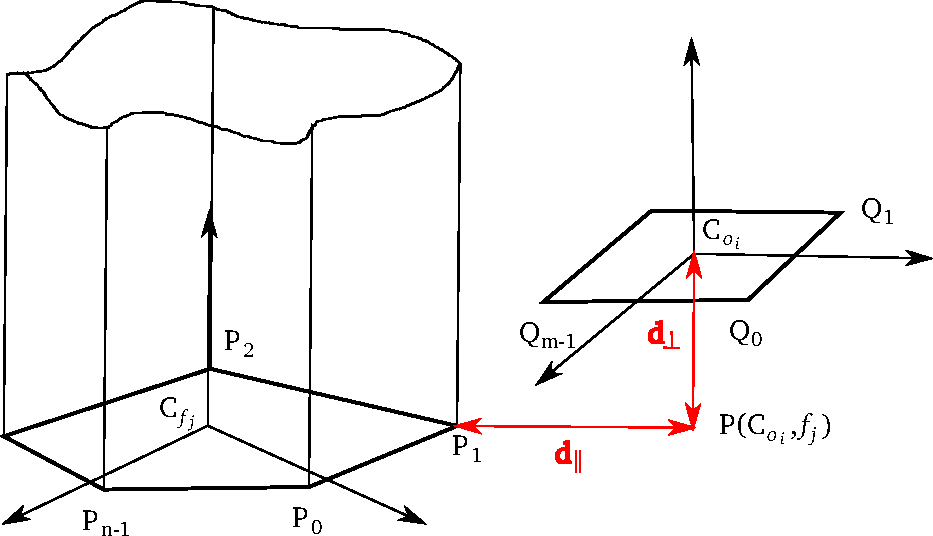
\includegraphics[width=\linewidth]{figures/convex-shape-contact.pdf}
  \end{center}
  \caption{Distance defined by two convex polygons.}
  \label{fig:convex-shape-contact}
\end{figure}

When an object is not grasped, it should lie in a stable pose. There are two simple methods to do that:
\begin{enumerate}
\item defining virtual grippers in the environment and virtual handles on the object, implicitely defines a discrete set of poses,
\item defining a virtual gripper on an horizontal plane and a virtual handle on the object, and using a grasp with flags $(\false,\false,\true,\true,\true,\false)$ constrains the object to move on a infinite horizontal plane.
\end{enumerate}

We propose here a third method that enables users to define contact surfaces in a more flexible way. In this aim, we denote by:
\begin{itemize}
\item $(o_i)_{i\in I}$ a set of convex polygons attached to an object,
\item $(f_j)_{j\in J}$ a set of convex polygons attached to the environment or to a mobile part of a robot that can receive objects (mobile robot for instance),
\item respectively $C_{o_i}$, $\mathbf{n}_{o_i}$ the barycenter of $o_i$ and the normal to the plane containing $o_i$,
\item $C_{f_j}$, $\mathbf{n}_{f_j}$ the barycenter of $f_j$ and the normal to the plane containing $f_j$,
\item $P(C_{o_i},f_j)$, the orthogonal projection of $C_{o_i}$ onto the plane containing $f_j$.
\end{itemize}
Then we define the distance between polygons $o_i$ and $f_j$ as the distance of $C_{o_i}$ to the cylindrical volume of generatrix $\mathbf{n}_{f_j}$ and of directrix $f_j$:
\begin{align}\label{eq:contact-distance}
  d(f_j,o_i) = \sqrt{d_{\parallel}^2 + d_{\perp}^2}
\end{align}
where
\begin{align*}
  i,j & \mbox{ are the indices that minimize the above distance,}\\
d_{\parallel} &= \left\{\begin{array}{lll} d(f_j,P(C_{o_i},f_j))&\mbox{if}& P(C_{o_i},f_j)\mbox{ outside } f_j\\
0 & & \mbox{otherwise}
\end{array}\right. \\
d_{\perp} &= \mathbf{n}_{f_j}.\vec{C_{f_j}C_{o_i}}.
\end{align*}
Figure~\ref{fig:convex-shape-contact} illustrates this notation.

We denote by $o_i(\conf)$ and $f_j(\conf)$ the poses in configuration $\conf$ of frames with respective centers $C_{o_i}$ and $C_{f_j}$ and with $x$-axis normal to each polygon. In an analogous way as in Definition~\ref{def:grasp}, we define
\begin{equation}\label{eq:convex-shape-contact-hbar}
\bar{h}(\conf) = \log_{\reals^3\times SO(3)} \left(f_{j}(\conf)^{-1}o_i(\conf)\right)
\end{equation}
The contact constraint is defined by the following piecewise differentiable function:
\begin{equation}\label{eq:convex-shape-contact}
h(\conf) = \left\{\begin{array}{lll}(\bar{h}_1,0,0,\bar{h}_4,\bar{h}_5)&
\mbox{if} & P(C_{o_i},f_j)\mbox{ inside } f_j\\
(\bar{h}_1,\bar{h}_2,\bar{h}_3,\bar{h}_4,\bar{h}_5)&
\mbox{if} & P(C_{o_i},f_j)\mbox{ outside } f_j\end{array}\right.
\end{equation}
It is straightforward that the above function vanishes if and only if two convex polygons are in contact.

As for grasps, we need to define a parameterized complement constraint for the contact constraint in order to specify the submanifold of configurations that are reachable from one configuration while keeping the object in a constant stable pose. The naive way consists in defining
$$
h_{comp}(\conf) = \left\{\begin{array}{lll}(\bar{h}_2,\bar{h}_3,\bar{h}_6)&
\mbox{if} & P(C_{o_i},f_j)\mbox{ inside } f_j\\
(0,0,\bar{h}_6)&
\mbox{if} & P(C_{o_i},f_j)\mbox{ outside } f_j\end{array}\right.
$$
$\bar{h}_2$, $\bar{h}_3$, $\bar{h}_6$ respectively represent the translation in $x-y$ plane and the rotation around $z$-axis of frame $o_i$ with respect to frame $f_j$. Let $\conf_0$ be a configuration such that $h(\conf_0)=0$. The submanifold defined by
\begin{equation}\label{eq:stable-pose}
\left\{\conf\in\CS,\ \ h(\conf)=0\ \ h_{comp}(\conf) = h_{comp}(\conf_0) \right\}
\end{equation}
contains one object pose for each pair of polygons $(o_i,f_j)$, and there are
$|I| . |J|$ possible combinations. This contraint is therefore not suitable to
enforce object immobility along a path since the object may jump from one pose to another one.

To disambiguate the various combination of convex polygons that can be in contact, we define
\begin{equation}\label{eq:convex-shape-contact-complement}
h_{comp}(\conf) = \left\{\begin{array}{l}(\bar{h}_2 + 2jM,\bar{h}_3 + 2iM,\bar{h}_6)\\
\mbox{if } P(C_{o_i},f_j)\mbox{ inside } f_j\\
(2jM,2iM,\bar{h}_6)\\
\mbox{if } P(C_{o_i},f_j)\mbox{ outside } f_j\end{array}\right.
\end{equation}
where
\begin{itemize}
\item $i$ and $j$ are the indices that minimize distance~(\ref{eq:contact-distance}),
\item $M$ is a positive real number such that for any $\kappa\in J$, all vertices of $f_\kappa$ are included in the disk of center $C_{f_\kappa}$ and of radius $M$.
\end{itemize}
With this definition, the submanifold defined by~(\ref{eq:stable-pose}), (\ref{eq:convex-shape-contact}), (\ref{eq:convex-shape-contact-complement}) contains configurations where the object is in a unique stable pose. The polygon indices $i$ and $j$, as well as their relative position can indeed be recovered from~(\ref{eq:convex-shape-contact-complement}):
\begin{align*}
  i &= \left\lfloor\frac{\bar{h}_3}{2M} + \frac{1}{2}\right\rfloor\\
  j &= \left\lfloor\frac{\bar{h}_2}{2M} + \frac{1}{2}\right\rfloor\\
  \bar{h}_1 &= \bar{h}_4 = \bar{h}_5 = 0\\
  \bar{h}_2 &= h_{comp\ 1} - 2jM\\
  \bar{h}_3 &= h_{comp\ 2} - 2iM\\
  \bar{h}_6 &= h_{comp\ 3}
\end{align*}
and from (\ref{eq:convex-shape-contact-hbar}),
$$
f_{j}(\conf)^{-1}o_i(\conf) = \exp_{\reals^3\times SO(3)}\left(\bar{h}\right).
$$
Uniqueness comes from the fact that when two convex polygons are in contact,
necessarily, $|\bar{h}_2| \leq M$,$|\bar{h}_3| \leq M$.
% Remark about convergence of the solver and about explicit constraint.

\subsection{constraint graph}

According to Definition~\ref{def:manipulation-problem}, the set of admissible configurations is the union of sub-manifolds of the configuration space of the system. Each sub-manifold is defined by grasp and/or stable contact constraints. We call each sub-manifold a \textit{state} of the problem. A state is defined by a set of grasps and a set of stable contact poses.

A state can be defined by a subset of active grasps, any object not grasped being in a stable contact pose. Let $\ngrippers$ and $\nhandles$ repsectively denote the number of grippers and handles. A state $\state$ is denoted by a vector of size $\ngrippers$:
\begin{equation}\label{eq:state}
\state = \left(h_1,\cdots,h_{\ngrippers}\right)
\end{equation}
where $h_i\in\{\emptyset,1,\cdots,\nhandles\}$ denotes the id of the handle grasped by gripper $i$; $h_i=\emptyset$ means that gripper $i$ does not grasp any handle.

\paragraph{Number of states:} note that for $i\in\{1,\cdots,\nhandles\}$ the number of occurences of $i$ in $\state$ is at most 1: a handle cannot be grasped by several grippers. Note also that the number of occurences of $\emptyset$ is not limited: several grippers may hold nothing. Let $m$ be a non-negative integer not greater than $\ngrippers$ and than $\nhandles$ and let us count the number of states with $m$ handles grasped. The number of subset of $m$ handles among $\nhandles$ is equal to $\frac{\nhandles!}{(\nhandles-m)!m!}$. And the number of ways of dispatching them among the $\ngrippers$ grippers is equal to $\frac{\ngrippers!}{(\ngrippers-m)!}$. Thus, the total number of states is equal to
$$
\sum_{m=0}^{\min(\ngrippers,\nhandles)} \frac{\nhandles!}{(\nhandles-m)!m!} \frac{\ngrippers!}{(\ngrippers-m)!}
$$
\begin{definition}\label{def:neighboring-states}\textbf{Neighboring states}\\
  Two states $\state_1=(h_{1 1},\cdots,h_{\ngrippers 1})$ and $\state_2=(h_{1 2},\cdots,h_{\ngrippers 2})$ are neighboring if they differ by only one grasp and the grasp is empty in one of the states:
  \begin{align*}
    &\exists i\in\{1,\cdots,\ngrippers\},\,h_{i 1} \not= h_{i 2} \mbox{ and } (h_{i 1}=\emptyset \mbox{ or } h_{i 2}=\emptyset), \mbox{ and }\\
    &\forall j\in\{1,\cdots,\ngrippers\},\, j\not=i,h_{j 1} = h_{j 2}.
  \end{align*}
\end{definition}
\begin{definition}\label{def:constraint-graph}\textbf{Constraint graph}\\
  The constraint graph related to a manipulation problem as defined in Definition~\ref{def:manipulation-problem} is a graph
  \begin{itemize}
  \item the nodes of which are states defined by subsets of grasps~(\ref{eq:state}),
  \item an edge connects two states if and only if they are neighboring or they are equal. Edges are also called \textit{transitions}.
  \end{itemize}
  Nodes contain
  \begin{itemize}
  \item the grasp constraints that are active in the corresponding state,
  \item a placement constraint for each object that is not grasped by any handle.
  \end{itemize}
  Transitions contain
  \begin{itemize}
  \item the constraints of the node they connect with the least active grasps,
  \item the parameterized complement constraint of each of the latter.
  \end{itemize}
\end{definition}

\subsection{Example}

\begin{figure}
  \begin{center}
    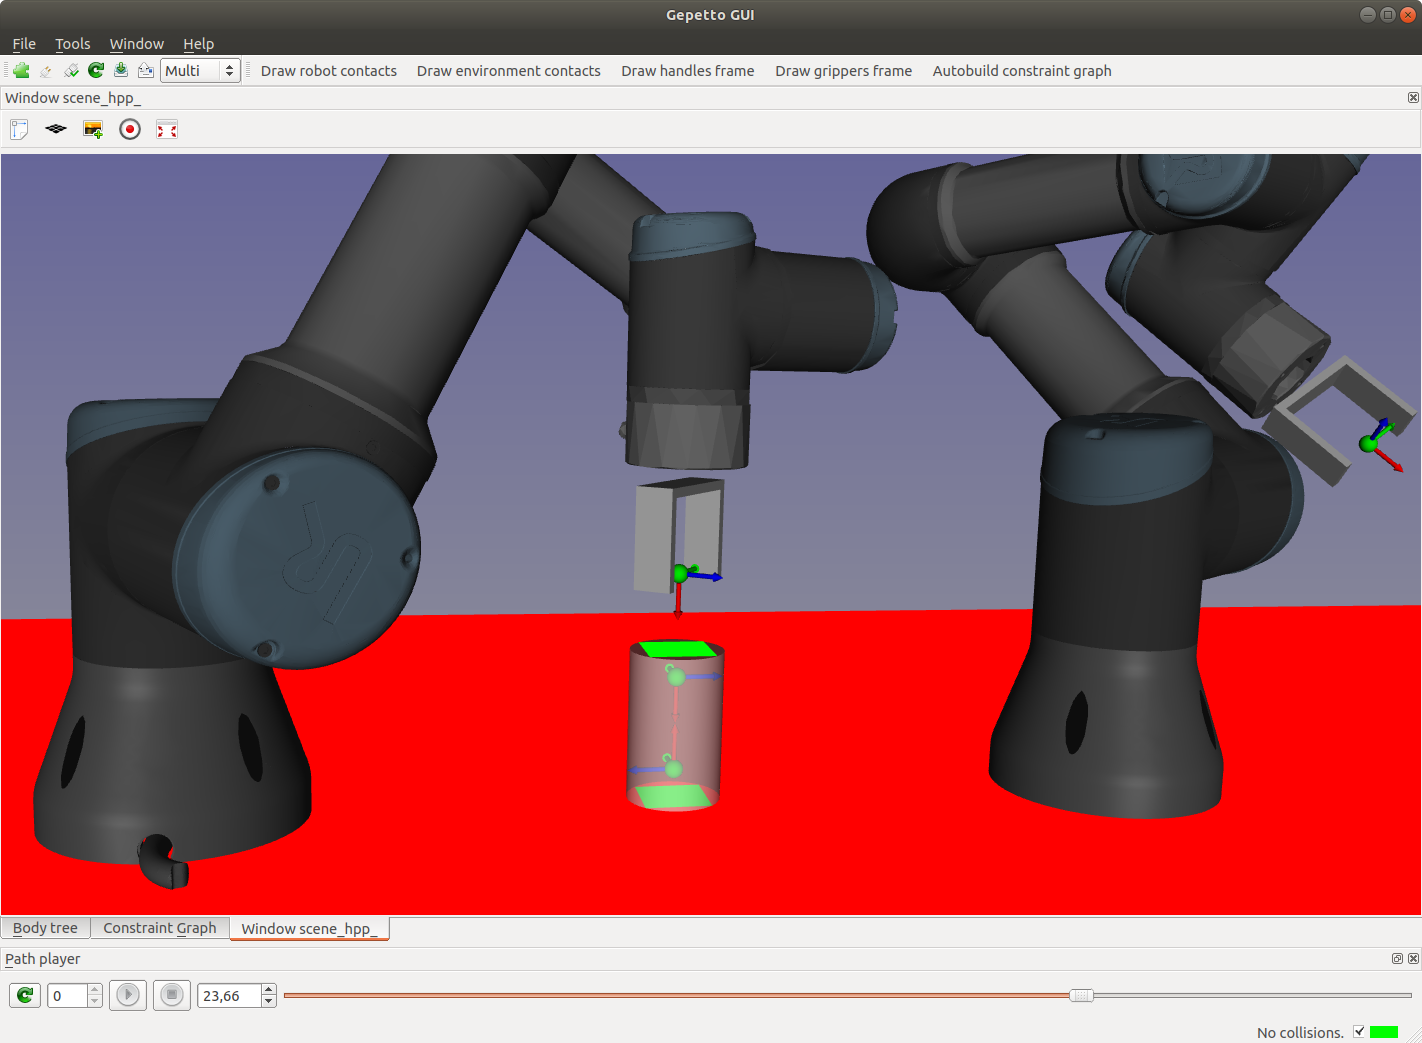
\includegraphics[width=\linewidth]{figures/example.png}
    \def\svgwidth{\columnwidth}
    \graphicspath{{./figures/}}
    \input{figures/example-graph.pdf_tex}
  \end{center}
  \caption{Top: two robot UR3 with one gripper each (X=red, Y=gree, Z=blue) manipulating a cylinder with two handles. The environment contains one rectangular contact surface (in red). The cylinder has two rectangular contact surfaces (in green).
  Bottom: the corresponding constraint graph. Names of states follow Expression~(\ref{eq:state}): for instance, $(\emptyset,1)$ means that gripper of robot 2 grasps handle 1 of the cylinder. In this state, there is no placement constraint.}
  \label{fig:2ur3-cylinder}
\end{figure}
To illustrate the notions exposed in the previous sections, let us consider an example of two UR3 robots manipulating a cylinder illustrated in Figure~\ref{fig:2ur3-cylinder}. The robot is equipped with one gripper attached to the end-effector. The cylinder is equipped with two handles and with two square contact surfaces corresponding to the top and bottom faces of the cylinder.

Grasp constraints are denoted by
$$
grasp_{ij} \mbox{ where } i,j\in\{1,2\}.
$$
Grasp complement constraints are denoted by
$$
grasp_{ij}/comp \mbox{ where } i,j\in\{1,2\}.
$$

$i$ is the index of the gripper $j$ is the index of the handle. The flag of the handles is
$$(\true,\true,\true,\false,\true,\true).$$
Therefore grasp constraints are of dimension 5 and keep the rotation of the gripper around the cylinder axis free.
The object placement constraint is denoted by $place$ and the complement by $place/comp$.
\begin{table}
  \begin{center}
    \begin{tabular}{|p{.44\linewidth}|p{.44\linewidth}|}
      \hline
      state & active constraints\\
      \hline
      $(\emptyset,\emptyset)$ & $place$ \\
      $(j,\emptyset),\,j\in\{1,2\}$ & $grasp_{1j}$\\
      $(\emptyset,j),\,j\in\{1,2\}$ & $grasp_{2j}$\\
      $(i,j)\,i,j\in\{1,2\}$ & $grasp_{1i},grasp_{2j}$\\
      \hline
    \end{tabular}
  \end{center}
  \caption{State constraints.}
  \label{tab:state-constraints}
\end{table}
Table~\ref{tab:state-constraints} indicates which constraints are active for each state.

\begin{table}
  \begin{center}
    \begin{tabular}{|p{.23\linewidth}|p{.18\linewidth}|p{.43\linewidth}|}
      \hline
      transition & belongs to & additional constraints\\
      \hline
      $(\emptyset,\emptyset)\rightarrow (i,\emptyset)$ & $(\emptyset,\emptyset)$ & $place/comp$\\
      $(\emptyset,\emptyset)\rightarrow (\emptyset,i)$ & $(\emptyset,\emptyset)$ & $place/comp$\\
      $(i,\emptyset)\rightarrow(i,j)$ & $(i,\emptyset)$ & $grasp_{1i}/comp$\\
      $(\emptyset,j)\rightarrow(i,j)$ & $(\emptyset,j)$ & $grasp_{2j}/comp$\\
      \hline
    \end{tabular}
  \end{center}
  \caption{Transition constraints: $i,j$ are either 1 or 2. column "belongs to" means that paths along the transition belong to the state.}
  \label{tab:transition-constraints}
\end{table}

\subsection{Automatic construction}

\begin{algorithm}
  \algblock[globalVariable]{GlobalVariable}{EndGlobalVariable}
  \begin{algorithmic}[1]
    \GlobalVariable
    \State{$\nobjects$}\Comment{number of objects}
    \State{$\ngrippers$}\Comment{number of grippers}
    \State{$\nhandles$}\Comment{number of handles}
    \EndGlobalVariable
    \Function{buildConstraintGraph}{}
    \State{$\mathcal{G}\gets\left[0,\cdots,\ngrippers-1\right]$}
    \Comment{gripper indices}
    \State{$\mathcal{H}\gets\left[0,\cdots,\nhandles-1\right]$}
    \Comment{handle indices}
    \State {$Gr\gets\left[\emptyset,\cdots,\emptyset\right]$}\Comment{list of size $\ngrippers$}
    \State \Call{recurse}{$\mathcal{G}$,$\mathcal{H}$,$Gr$}
    \EndFunction
    \Function{recurse}{$\mathcal{G}$,$\mathcal{H}$,$Gr$}
    \State\Call{createState}{$Gr$}
    \If{$\mathcal{G}=\emptyset$ or $\mathcal{H}=\emptyset$}
    \State{\Return}
    \EndIf
    \For{$g$ in $\mathcal{G}$}
    \State{$\mathcal{G}^{\prime}\gets \mathcal{G}\setminus\{g\}$}
    \For{$h$ in $\mathcal{H}$}
    \State{$\mathcal{H}^{\prime}\gets\mathcal{H}\setminus\{h\}$}
    \State{$Gr^{\prime}\gets Gr$}
    \State{$Gr^{\prime}[g]\gets h$}
    \State{\Call{createState}{$Gr^{\prime}$}}
    \State{\Call{createTransition}{$Gr$, $Gr^{\prime}$}}
    \State{\Call{recurse}{$\mathcal{G}^{\prime}$,$\mathcal{H}^{\prime}$,$Gr^{\prime}$}}
    \EndFor
    \EndFor
    \EndFunction
    \Function{createState}{$Gr$}
    \If{\Call{existState}{$Gr$}}\State{\Return}\EndIf
    \State{$\state\gets\mbox{ new state}$}
    \State{$\state.Pl\gets\left[\true,...,\true\right]$}\Comment{list of size $\nobjects$}
    \For{$g\mbox{ in } \left[0,\cdots,\ngrippers-1\right]$}
    \State{$h\gets Gr[g]$}
    \State{$\state.Pl[\Call{objectIndex}{h}]\gets\false$}
    \State{$\state$.add(\Call{graspConstraint}{g,h})}
    \EndFor
    \For{$o\mbox{ in }\left[0,\cdots,\nobjects\right]$}
    \If{$\state.Pl[o]$}
    \State{$\state$.add(\Call{placeConstraint}{$o$}})
    \EndIf
    \EndFor
    \EndFunction
    \Function{createTransition}{$Gr_1,Gr_2$}
    \State{$\transition\gets\mbox{ new transition}(Gr_1,Gr_2)$}
    \State{$\state_1\gets$\Call{state}{$Gr_1$}}\Comment{Recover state for this set of grasps}
    \For{$g\mbox{ in } \left[0,\cdots,\ngrippers-1\right]$}
    \State{$h\gets Gr_1[g]$}
    \State{$\transition$.add(\Call{graspConstraint}{g,h})}
    \State{$\transition$.add(\Call{graspConstraintComp}{g,h})}
    \EndFor
    \For{$o\mbox{ in }\left[0,\cdots,\nobjects\right]$}
    \If{$\state_1.Pl[o]$}
    \State{$\transition$.add(\Call{placeConstraint}{$o$}})
    \State{$\transition$.add(\Call{placeConstraintComp}{$o$}})
    \EndIf
    \EndFor
    \EndFunction
    \Function{existState}{$Gr$}
    \Comment{Return $\true$ if a state has already been created for the set of
    grasps given as input.}
    \EndFunction
    \Function{state}{$Gr$}
    \Comment{Return the state created with the set of grasps given as input.}
    \EndFunction
    \Function{objectIndex}{$h$}
    \Comment{Return the index of the object handle $h$ belongs to.}
    \EndFunction
  \end{algorithmic}
  \caption{Recursive Construction of the constraint graph. The
    construction starts by the state with no grasp. Call to recurse
    function loops over the available grippers and handles and create
    states with one more grasp, and a transition to these new
    states. In each state, a placement constraint is added for each
    object of which no handle is grasped. Variables $\mathcal{G}$ and
    $\mathcal{H}$ contain the indices of the free grippers and
    handles. Variable $Gr$ stores the current set of grasps following
    Expression~(\ref{eq:state}). Functions {\scriptsize GRASP}{\small C}{\scriptsize ONSTRAINT}, {\scriptsize GRASP}{\small C}{\scriptsize ONSTRAINT}{\small C}{\scriptsize OMP},{\scriptsize PLACE}{\small C}{\scriptsize ONSTRAINT}, {\scriptsize PLACE}{\small C}{\scriptsize ONSTRAINT}{\small C}{\scriptsize OMP} build grasp, placement constraints and their complements as defined in sections~\ref{subsec:grasp} and ~\ref{subsec:placement}.}
  \label{algo:constraintGraphFactory}
\end{algorithm}

Given a set of grippers, handles and objects, the constraint graph can be constructed automatically. \href{https://github.com/humanoid-path-planner/hpp-manipulation-corba/blob/5af1b3bad68e8c339d5f42eb72173d7356504532/src/hpp/corbaserver/manipulation/constraint_graph_factory.py#L187}{Here} is an implementation in python. Algorithm~\ref{algo:constraintGraphFactory} describes this implementation.

\section{Manipulation planning}

In this section, we show how the constraint graph defined in the previous section is used to plan collision-free manipulation paths. Although we are working on an extension of Algorithm RMR*~\cite{schmitt17icra} to several grippers, objects and handles, the only manipulation planning algorithm available up to now in HPP is an extension of RRT algorithm described in the next section.

\subsection{M-RRT}

Manipulation Randomly exploring Random Tree is an extension of RRT algorithm~\cite{LavKuf01b} that grows trees in the free configuration space, exploring the different states of the manipulation problem. Algorithm~\ref{algo:M-RRT} describes the algorithm implemented \href{https://github.com/humanoid-path-planner/hpp-manipulation/blob/16369aa291ab1b17ef6176ae8b8b2512b5e6fff7/src/manipulation-planner.cc#L159}{here}.
\begin{algorithm}
  \begin{algorithmic}[1]
    \Function{oneStep}{}
    $q_{rand}\gets$\Call{randomConfig}{}
    \EndFunction
  \end{algorithmic}
  \caption{}
  \label{algo:M-RRT}
\end{algorithm}

\subsection{Waypoint edges}

\subsection{Crossed foliation issue}

\subsection{Prototyping dedicated algorithms}



\begin{acknowledgements}
This work has been partially supported by Airbus S.A.S. in the framework of the common laboratory Rob4Fam.
\end{acknowledgements}


% Authors must disclose all relationships or interests that 
% could have direct or potential influence or impart bias on 
% the work: 
%
% \section*{Conflict of interest}
% The authors declare that they have no conflict of interest.


% BibTeX users please use one of
\bibliographystyle{spbasic}      % basic style, author-year citations
%\bibliographystyle{spmpsci}      % mathematics and physical sciences
%\bibliographystyle{spphys}       % APS-like style for physics
%\bibliography{}   % name your BibTeX data base

% Non-BibTeX users please use
\bibliography{hpp}

\end{document}
% end of file template.tex

